In the previous chapter we showed that interferometric detectors, such
as LIGO, are capable of encoding the presence of gravitational waves
in the phase shifts of light.  These shifts over time, or rather the
motion of the servos to prevent them, are recorded as the data stream
\darmerr.  As noted, this data stream will also contain noise.  This
noise will contain both a continuous component which sets the overall
sensitivity of the detector, and short glitches which can interfere
with the search.

In this chapter we discuss a method to extract signals, if present,
from the noise and hence allow the LIGO and Virgo collaborations to
claim a direct detection of gravitational waves.  For the most part in
this chapter we will disregard implementation details.  In particular,
we will treat quantities as continuous in both time and magnitude.  In
reality the data is sampled at 16384 Hz, and all time integrals
should be replaced by sums.  Values are also stored in a discrete
form, although the resolution is no coarser than the resolution of
IEEE floating-point numbers.  Analysis codes therefore do not need any
special features to deal with this discretization, beyond the usual
care taken not to accumulate numerical errors.  In particular, Fourier
transforms, special functions, and similar functionality can be
provided by standard code libraries.



\section{Detecting Signals in Noise}
\label{sec:ihope_match_filter}

There are many ways to search for evidence of gravitational waves in
noise and to a large extent the method used will depend on the nature
of the signal being sought.  In this chapter we focus on \emph{matched
filtering}, which is optimal given certain assumptions about the noise
and if we have an accurate model of the signal for which we are
searching.  Such a method is ideal for searching for the coalescence
of compact binaries, as discussed in chapter~\ref{ch:theory}, as we
can use the analytic approximations as the model.  The question of how
well these models match real signals then becomes critical, and 
we will return to this question in subsequent chapters.

\subsection{Random Processes}
\label{ssec:random_processes}

We start by modelling the noise in the instruments, following the
treatment in~\cite{BlandfordThorne}.  Seismic noise is not predictable
in any detailed way, and thermal and shot noise are quantum-mechanical
in nature and therefore can not be predicted even in principle.  The
noise is therefore a \emph{random process}.  Such a process is
described by a collection of probability density functions of the form

\begin{equation*}
\label{eq:pdfs}
p(y_n, t_n; y_{n-1}, t_{n-1}; \ldots y_0 t_0) dy_n dy_{n-1} \ldots
dy_0
\end{equation*}

which gives the probability that the value at time $t_0$ will will
lie between $y_0$ and $y_0 + dy_0$ and that the value at time $t_1$
will will lie between $y_1$ and $y_1 + dy_1$, and so on.

By considering a hypothetical ensemble of such processes we can
construct average values of functions of the process at one or more
times.  We denote the ensemble average of a quantity $x$ by angle
brackets, $\langle x \rangle$, for example the average value of the product
$y(t_1)y(t_2)$ is
%
\begin{equation*}
\langle y(t_1) y(t_2) \rangle = \int y_2 y_1
p(y_2, t_2; y_1, t_1)\, dy_2\, dy_1
\end{equation*}

We now make the following assumptions about the LIGO noise:
%
\begin{itemize}
\item That it is \emph{stationary}, the values of the
functions~\ref{eq:pdfs} depend only on the differences between the
times, and not any absolute external clock.  This is not necessary a
good model for seismic noise, but by breaking the analysis into small
chunks of time it will be accurate enough over the span of each.

\item That it is \emph{Gaussian}, that is, the functions~\ref{eq:pdfs}
are all of the form $\exp(-Y^T A Y)$ where $Y$ is a vector of $y$
values and  $A$ is a positive-definite matrix.  This is not
necessarily a good model for, eg, electrical noise, which is better
modeled as a sine wave with time-dependant random amplitude.  This is
definitely not a good model for the numerous non-Gaussian glitch
mechanisms.  However, this assumption is again approximately correct.  We
will further assume that the mean is 0 (eg, that the mirrors are just
as likely to swing one way as the other).

\item That it satisfies the \emph{ergodic hypothesis} so that we may
replace ensemble averages with time averages.

\end{itemize}

Now consider the quantity $S_y(f)$ called the \emph{power spectral
density} (PSD), defined as

\begin{equation}
\label{eq:psd1}
S_y(f) \equiv \lim_{T \to \infty} 
\frac{1}{T} \left| \int_{-T/2}^{T/2} (y(t) - \bar{y}(t))
e^{2 \pi i f t} dt \right|^2
\end{equation}
%
Using Parceval's theorem it can be shown that
%
\begin{equation*}
\int_0^\infty S_y(f)\, df = \sigma^2_y
\end{equation*}
%
That is, $S_y(f)$ measures the contribution of each frequency 
to the total variance of the process.
%
It can also be shown that 
%
\begin{equation}
\label{eq:psd2}
\langle \tilde{y}(f) \tilde{y}(f')\rangle = \frac{1}{2} S_y(f)
\delta(f-f')
\end{equation}

\subsection{The Matched Filter}
\label{ssec:matched_filter}

We now specialize to the case of LIGO.  We denote the noise in the
detector as $n(t)$, and a gravitational-wave signal as $h(t)$.  The
output of the detector is then $s(t)=n(t)+h(t)$.  We seek a filter on
the data that we can use to infer the presence of the signal.

Consider the most general linear filter which in the discrete case
would be
%
\begin{equation}
\hat{s} = \sum_i s_i K_i
\end{equation}
%
Since we will want a real result, we require the $K_i$ to be real.  In
the continuum limit this becomes
%
\begin{equation}
\hat{s} = \int_{-\infty}^\infty s(t) K(t)\, dt
\end{equation}

We now define the signal strength $S$ as the expected value of
$\hat{s}$ when the signal is present:
%
\begin{align*}
S &= \left\langle \hat{s} \right\rangle \\
&= \left\langle  \int_{-\infty}^\infty s(t) K(t)\, dt \right\rangle \\
&= \int_{-\infty}^\infty \langle s(t) K(t)\rangle \, dt \\
&= \int_{-\infty}^\infty \langle s(t) \rangle K(t) \, dt \\
&= \int_{-\infty}^\infty \langle n(t) + h(t) \rangle K(t) \, dt \\
&= \int_{-\infty}^\infty \left( \langle n(t) \rangle + \langle h(t)
\rangle \right)  K(t) \, dt \\
&= \int_{-\infty}^\infty \left( 0 + h(t) \right)  K(t) \, dt \\
&= \int_{-\infty}^\infty h(t) K(t) \, dt \\
\end{align*}
%
Now, since $K(t)$ is real we can replace it by its complex conjugate
and then apply Parseval's theorem to write this as
%
\begin{equation*}
S = \int_{-\infty}^\infty h(t) K^\star(t) \, dt
= \int_{-\infty}^\infty \tilde{h}(f) \tilde{K}^\star(f) \, df
\end{equation*}

We characterise the noise $N$ as the rms value of $\hat{s}$ when the
signal is absent:
%
\begin{align}
N^2 &= \langle \hat{s}^2(t) \rangle - \langle \hat{s}(t) \rangle^2 \\
&= \langle \hat{s}^2(t) \rangle  \\
&= \int_{-\infty}^\infty K(t) K(t') \langle n(t) n(t')
\rangle\,dt\,dt' \\
&= \int_{-\infty}^\infty dt\,dt' K(t) K(t') 
\int_{-\infty}^\infty df\,df' e^{2\pi i f t}e^{-2\pi i f' t'} \langle
\tilde{n}^\star(f) \tilde{n}(f')\rangle \\
\end{align}
%
Using Eqn.~\ref{eq:psd2} this becomes
%
\begin{equation}
N^2 = \int_{-\infty}^\infty df\,\frac{1}{2} S_n(f) |\tilde{K}(f)|^2
\end{equation}

We now introduce a new function
%
\begin{equation}
\tilde{u}(f) = \frac{1}{2} S_n(f) \tilde{K}(f)
\end{equation}
%
In terms of which we can write the signal-to-noise ratio, which we
henceforth denote as $\rho$ as
%
\begin{equation}
\rho =
\frac
  {\int_{-\infty}^\infty df\,
   \frac
     {\tilde{h}(f) \tilde{u}^\star(f)}
     {(1/2) S_n(f)}}
  {\left[\int_{-\infty}^\infty df\,
   \frac
     {\tilde{u}(f) \tilde{u}^\star(f)}
     {(1/2) S_n(f)}\right]^{1/2}}
\end{equation}

This motivates the definition of an operator mapping pairs of
functions to real numbers
%
\begin{equation}
\label{eq:InnerProduct}
\InnerProduct{A|B} 
 = 2 \int_{-\infty}^\infty df\,
   \frac
     {\tilde{A}(f) \tilde{B}^\star(f)}
     {S_n(f)}
\end{equation}
%
This operator has the following properties
%
\begin{itemize}
\item Conjugate symmetry, $(x|y) = (y|x)^\star$
\item Linearity in the first argument $(ax + by|z) = a(x|z) + b(y|z)$ for
$a,b$ numbers and $x,y,z$ functions.  This follows from the linearity
of the Fourier transform.
\item Positive-definiteness $(x|x) \geq 0$ and $(x|x) = 0$ iff $x=0$.  This
follows from the positive-definiteness of the product $aa^\star$ for
$a \in \mathcal{C}$.
\end{itemize}
%
The operator has all the properties of an inner product on
the vector space of functions.  We may therefore consider
%
\begin{equation*}
\frac{u}{(u|u)}
\end{equation*}
%
to be a normalized vector.

An important feature of this inner product, which we will use
repeatedly, is that the probability of obtaining any particular 
pattern $h(t)$ in the data is, up to normalization~\cite{Finn1992},
%
\begin{equation}
\label{eq:prob_of_signal}
p(h) \propto \exp\left(- \frac{1}{2} \InnerProduct{h|h} \right)
\end{equation}

Now using Eqn.~\ref{eq:InnerProduct} the SNR becomes
%
\begin{equation}
\label{eq:InnerProductSNR}
\rho = \frac{\InnerProduct{h|u}}{\InnerProduct{u|u}^{1/2}}
\end{equation}
%
We next seek a function $u$ (and hence $K$) that will maximize $\rho$.
In this form it is clear that $u$ and $h$ must be parallel, and
therefore
%
\begin{equation}
\tilde{K}(f) \propto \frac{\tilde{h}}{S_n(f)}
\end{equation}
%
The constant cancels, and may therefore be set to 1.

Combining these results, the value we will use to determine whether or
not our data $s$ contains the gravitational waveform $h$ (henceforth
called the \emph{template} waveform) is
%
\begin{equation}
\label{eq:snr}
\rho = \frac{\InnerProduct{s|h}}{\sqrt{\InnerProduct{h|h}}}
\end{equation}

The template has an unknown phase, denoted $\phi_0$ in
Eqn.~\ref{eq:spa_waveform}.  As this term has no frequency
dependence it gives rise to a constant of the form $\exp(i\phi_0)$,
which can be pulled out of the integral.  We can then maximize over
this value by taking the absolute value. 

The result is valid for a segment of data of length $t$ seconds
and a waveform of the same length.  However, there may be a signal in
the data that does not end where the template does. We should
therefore evaluate~\ref{eq:snr} repeatedly, sliding the template so
that it ends at a different time for each iteration.  However, this
can be done in a single operation.  If $\tilde{h}(f)$ is the Fourier
transform of $h(t)$, then the Fourier transform of $h(t+\tau)$ is
%
\begin{equation*}
\tilde{h}(f)' = \int h(t+\tau) e^{2 \pi i f t} dt
= \int h(t') e^{2 \pi i f (t'-\tau)} dt'
= e^{-2 \pi i } \tilde{h}(f)
\end{equation*}
%
Substituting this into the matched filter,
%
\begin{equation}
\label{eq:snr_time_series}
\rho(\tau) = \frac{2}{\sqrt{\InnerProduct{h|h}}}
\left\lvert \int e^{-2\pi i f \tau} \frac{\tilde{s}(f)
\tilde{h}^\star(f)}{S_n(f)}\,df \right\rvert
\end{equation}
%
where we have added the absolute value from the maximization over
$\phi_0$.  This is just the inverse Fourier transform of the quantity
$\tilde{s}(f)\tilde{h}(f)^\star/S_n$.  

\subsection{The Overlap}
\label{ssec:overlap}

Consider data consisting of noise and a signal $h$.  Let $\rho$
be the SNR obtained by filtering this data with template $h$.  Then
the loss in SNR incurred by filtering with an incorrect template, $h'$
is
%
\begin{align}
\label{eq:motivate_overlap}
\rho - \rho' 
&= \frac{\InnerProduct{s|h}}{\sqrt{\InnerProduct{h|h}}}
- \frac{\InnerProduct{s|h'}}{\sqrt{\InnerProduct{h'|h'}}} \\ \nonumber
&= \frac{\InnerProduct{n|h}}{\sqrt{\InnerProduct{h|h}}}
+ \frac{\InnerProduct{h|h}}{\sqrt{\InnerProduct{h|h}}}
- \frac{\InnerProduct{n|h'}}{\sqrt{\InnerProduct{h'|h'}}}
- \frac{\InnerProduct{h|h'}}{\sqrt{\InnerProduct{h'|h'}}} \\
  \nonumber
\end{align}
%
Taking the mean of both sides the first and third terms vanish because
%
\begin{equation*}
\left\langle \InnerProduct{s|h} \right\rangle
= 2 \int_{-\infty}^\infty df\,
   \frac
     {\langle \tilde{n}(f) \rangle \tilde{h}^\star(f)}
     {S_n(f)}
= 0
\end{equation*}
%
where the last step follows from our assumption that the noise is
Gaussian with zero mean.  Equation~\ref{eq:motivate_overlap} then
becomes
%
\begin{align*}
\langle \rho - \rho'  \rangle
&= \frac{\InnerProduct{h|h}}{\sqrt{\InnerProduct{h|h}}}
- \frac{\InnerProduct{h|h'}}{\sqrt{\InnerProduct{h|h'}}} \\
&= \sqrt{\InnerProduct{h|h}} \left(1 -
\frac{\InnerProduct{h|h'}}{\sqrt{\InnerProduct{h|h}
\InnerProduct{h'|h'}}} \right)
\end{align*}

This motivates the definition of the \emph{overlap} between two waveforms $h$ and
$h'$ with respect to a given PSD,
%
\begin{equation}
  \label{eq:OverlapDefinition}
  \Overlap{h|h'} \equiv \frac{\InnerProduct{h|h'}}{
    \sqrt{\InnerProduct{h|h} \InnerProduct{h'|h'}}}
\end{equation}
%
which is a measure of how similar the two waveforms are, or conversely
how dissimilar they are and hence the fractional SNR we can expect to
lose using one rather than the other.  We will use this repeatedly in
subsequent chapters.


\subsection{Trigger Selection}
\label{ssec:analysis_trigger_selection}

From the SNR time series, $\rho(t)$ we wish to select \emph{triggers},
discreet points whose time and $\rho$ value correspond to the time and
significance of a potential detection.
Equation~\ref{eq:prob_of_signal} says that even in the absence of a
signal there will be random fluctuations in $\rho(t)$.  We therefore
require a threshold on $\rho(t)$ that will eliminate most of the
triggers arising from random fluctuations, but not so high as to
prevent detection of realistic signals.  LIGO has chosen 5.5 as this
threshold.  However, it is unnecessary and would be wasteful to create
a trigger from every point of $\rho(t)$in excess of this threshold.
$\rho(t)$ may be thought of as ``sliding'' the template against the
signal.  As the two line up $\rho(t)$ will increase, achieving a
maximum when they are perfectly aligned, and then decreasing.  We
therefore need only create a trigger from the largest value of
$\rho(t)$.  Since glitches can also elevate the $\rho(t)$, and indeed
may have larger values than real signals we can not simply take the
largest value across the entire analysis but must instead choose a
\emph{window}.  A logical choice for the length of this window is the
time length of the template.  For pN waveforms described in
Sec.~\ref{sec:PNWaveforms} this is defined as the time from which
the instantaneous frequency is 40 Hz to the time where it becomes
infinite.

The full trigger selection algorithm is:
\newpage

\begin{alltt}
for each sample point j
  if \(\rho\sb{j}\) > threshold
    if there is no event yet
      event\_start = j
      event\_snr   = \(\rho\sb{j}\)
    else if \(\rho\sb{j}\) > event\_snr
      event\_start = j
      event\_snr = \(\rho\sb{j}\)
    else if (j - event\_start) == template length
      record event
      event\_start = j
      event\_snr   = \(\rho\sb{j}\)
\end{alltt}
%
This is illustrated in Fig.~\ref{f:snr_cartoon}.  We will discuss
some implications of this algorithm in
Sec.~\ref{sec:daily_ihope_open_questions}.


\begin{figure}
  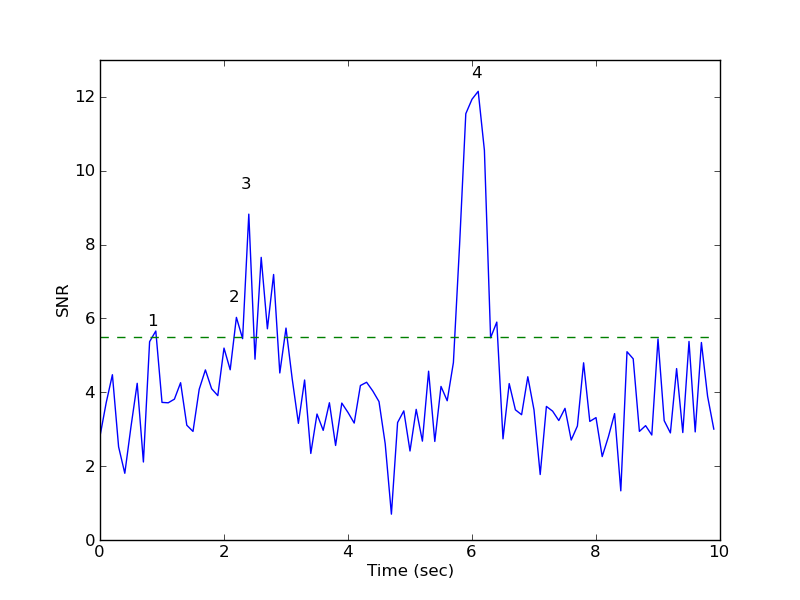
\includegraphics[width=\linewidth]{figures/search/snr_cartoon}
  \caption[The trigger-selection algorithm]{
  \label{f:snr_cartoon}
A ``cartoon'' illustrating the trigger-selection algorithm.  The graph
shows an SNR time series of the kind produced by
Eqn.~\ref{eq:snr_time_series}.  Assume the template is one second
long.  As the SNR rises above threshold just before point (1) the
``window'' opens.  Point (1) is found as the nearest maximum.  One
second after point (1) the window closes and point (1) is 
recorded as a trigger.  The SNR rises above threshold just
before point point (2).  This is more than one second away from point
(1), so a new window opens.  When point (3) is encountered it is
recorded as the largest value, resetting the window.  One second after
point (3) the window closes and point (3) is recorded as a trigger.
The two peaks following point (3) are within the one-second window,
they are not recorded as triggers.  Point (4) is likewise recorded as
a trigger, as it is more than one second from (3).
}
\end{figure}%



\section{The $\chisq$ Test}
\label{sec:ihope_chisq}

Consider again the SNR time series, Eqn.~\ref{eq:snr_time_series},
which we now write as
%
\begin{equation*}
\rho(t) = \frac{1}{\sqrt{\InnerProduct{h|h}}}
\int e^{-2\pi i f t} \frac{\tilde{h}^\star(f)}{S_n(f)} \cdot \tilde{s}(f) \,df
\end{equation*}
%
By the convolution theorem this becomes
%
\begin{equation*}
\rho(t) = \frac{1}{\sqrt{\InnerProduct{h|h}}}
h(-t) \star S(t) \star s(t)
\end{equation*}
%
where $S(t)$ is the inverse Fourier transform of $1/S_n(f)$.  If the
signal is an impulse, $s(t) = \delta(t)$, then the response is the
time-reversed template (``fuzzed'' by the noise curve).  Given a sharp
feature in the data the SNR will therefore be elevated, even though
the data looks nothing like a gravitational wave.  More
generally this demonstrates that the SNR alone is not
sufficient to distinguish signals from noise in the presence of
non-Gaussian features of the data.  Given the presence of glitches
this is a very practical concern.

We therefore supplement the analysis with a $\chisq$
signal-consistency test~\cite{Allen:2004}.  The idea is to check not
only that $\rho$ is large, but also that the SNR was accumulated over the
frequency integration in a way consistent with a real signal.  We do
this by dividing the template into $p$ sub-templates $h_i$, which
match the original template between frequencies $f_i$ and $f_{i+1}$
and are zero elsewhere and the $f_i$ are chosen such that
%
\begin{equation*}
\int_{f_i}^{f_{i+1}} \frac{|h_i|^2}{S_n(f)}\,df
= \frac{1}{p}
\int_{f_0}^{f_c} \frac{|h|^2}{S_n(f)}\,df
\end{equation*}
%
where $f_0$ is the starting frequency (40 Hz in LIGO) and $f_c$ is, as
in Eqn.~\ref{eq:spa_waveform}, the frequency at which we terminate
the waveform.  We then filter with these sub-templates independently
to produce the $p$ time series $\rho_i(t)$ and construct the quantity
%
\begin{equation}
\label{eq:chisq}
\chi^2(t) = p \sum_{i=1}^p \left(\rho_i(t) - \frac{\rho(t)}{p}\right)^2
\end{equation}
%
If the signal exactly matches the template $\chi^2$ will be zero, and
it will increase as the signal and template deviate.  Based on
investigations in S5, we choose $p=16$.

We incorporate this information in the analysis by constructing a
quantity, $\newsnr$ (new SNR), which downweights the SNR by $\chisq$,
%
\begin{equation}
\label{eq:new_snr}
\newsnr^2 = \begin{cases}
 \rho^2, & \chi^2_{r} \leq 1, \\ 
 \frac{\rho^2}{[(1+(\chi_r^2)^3)/2]^{1/6}}, \ & \chi^2_{r} > 1,
\end{cases}  
\end{equation}
%
where the first clause is added to avoid promoting triggers that
happen to have anomalously low $\chisq$ values, and the form and
factors of the second clause have been chosen based on studies to test
the ability of the search to distinguish between simulated injected
signals and glitches.

\section{Choosing the Templates}
\label{sec:bank_metric}

We have thus far referred to the $h$ as ``the template'', but recall
from Eqn.~\ref{eq:spa_waveform} that the waveforms depend on
the parameters of the binary, such as total mass $M$ and symmetric
mass ratio $\eta$.  As discussed in Sec.~\ref{ssec:overlap},
the difference between the signal and the template used in the matched filter 
corresponds directly to a reduction in $\rho$.  We must therefore
construct a \emph{bank} of templates arranged to capture, to within
some acceptable loss of SNR, all the signals of interest.  To do so we
consider the space of templates as a manifold, as in
chapter~\ref{ch:theory}, and we use the parameter values (or functions
of these values) as coordinates.  The distance between two points
$\mathbf{p}$ and $\mathbf{q}$, with coordinates=parameters $p_i$ and
$q_i$, is defined in terms of the overlap of templates at those
parameters
%
\begin{equation*}
d = 1 - \Overlap{h(\mathbf{p})|h(\mathbf{q})}
= \frac{\InnerProduct{h(\mathbf{p})|h(\mathbf{q})}}{
    \sqrt{\InnerProduct{h(\mathbf{p})|h(\mathbf{p})}
\InnerProduct{h(\mathbf{q})|h(\mathbf{q})}}}
\end{equation*}
%
We then seek a set of templates, $\{h_i\}$ such that within a region
of interest every point in the manifold is ``sufficiently close'' to
at least one template:
%
\begin{equation*}
\forall \mathbf{p}, \max_i \Overlap{h(\mathbf{p})|h_i} \geq x
\end{equation*}
%
Such a bank will ensure that the loss in SNR from using the bank
instead of testing the entire continuum of parameters is less than
$x\%$.  In LIGO we typically require no more than a 3\% loss in SNR.
As the distance to which we can detect signals scales with SNR and
volume is the cube of distance, this corresponds to approximately a
10\% loss in event rate.

It is possible to construct the bank
\emph{stochastically}~\cite{PhysRevD.80.104014}:

\begin{itemize}
\item Choose a point in the manifold at random

\item If the overlap with any already-placed template is greater than the
minimal match, discard it

\item Otherwise, add it to the set and continue

\item Repeat until there have been $N$ consecutive rejected new
candidates, where $N$ is chosen to give a reasonable probability that
the space has been covered.
\end{itemize}

In many cases however we can do better then this.  Since we are
interested in distances on a manifold it makes sense to seek a metric
on this space.  Such a metric can be obtained by expanding the
overlap function~\cite{Owen:1995tm, Owen:1998dk}

\begin{equation*}
\label{eq:bank_matric}
\Overlap{h(\mathbf{\lambda})|h(\mathbf{\lambda} +
\Delta\mathbf{\lambda})}
\approx 1 - \frac{1}{2} 
\frac{\partial^2 \Overlap{h(\mathbf{\lambda})|h(\mathbf{\lambda} +
\Delta\mathbf{\lambda})}}{\partial \Delta \lambda_i \partial \Delta \lambda_j}\bigg|_{\Delta
\mathbf{\lambda}=0} (\Delta
\lambda_i) (\Delta \lambda_j)
\end{equation*}
%
where we can drop the linear term because the overlap is a maximum at
$\Delta \mathbf{\lambda} = 0$.  When using frequency-domain,
stationary-phase templates of the form~\ref{eq:spa_waveform}, the
calculation of this metric can be done analytically, and gives a
result in terms of moments of the noise curve
%
\begin{equation*}
I(q) = S_n(f_0) \int_{f_0}^{f_c} \frac{x^{-q/3}}{S_n(x f_0)}\,dx
\end{equation*}
%
where $f_0$ is a chosen reference frequency.

The metric can then be used to efficiently lay out a grid of
templates.  In general it is impossible to lay out a grid on a curved
surface such that every point is the same distance from its nearest
neighbors, but the metric on the template manifold is approximately
flat and, when written in appropriate coordinates, the coefficients
are constant.


\section{The Search Pipeline}
\label{sec:search_pipeline}

We now discuss how the above elements are incorporated into a
gravitational-wave search.  The system is collectively known as a
\emph{pipeline}, as it may be thought of as a series of steps through
which the data flows.  In particular the LIGO-Virgo search for
gravitational waves from the coalescence of compact binaries is called
the \emph{ihope} pipeline.  There is a large gap between the basic
principles outlined above and a functioning gravitation-wave search.
More details can be found in
Refs.~\cite{Allen:2005fk,Allen:2004,Robinson:2008,hexabank}.  We now
present a very high-level overview of how these elements were used in
the search for gravitational waves from the coalescence of compact
binaries.  We focus in particular on LIGO's sixth science run which
overlaps Virgo's second and third.  For more details on this search
see Ref.~\cite{Capano:thesis}.

In the first step the data from each IFO the analysis is broken into
2048-second segments.  This is done for computational efficiency, as
well as to restrict to timespans over which the PSD is nearly
stationary.  Next, we filter to remove power below 40 Hz.  This is
done because computers are able to store numbers with only finite
range and precision.  In particular we are unable to small differences
above large values without losing information.  As the seismic noise
below 40 Hz is orders of magnitude greater than the noise at higher
frequencies signals at higher frequencies would be completely lost due
to rounding errors.

The PSD for each IFO is then calculated by a variation of
\emph{Welch's method}.  The 2048 seconds are split into 15 256-second
chunks, overlapping by 128 seconds.  The PSD of each chunk is then
calculated using the defining Eqn.~\ref{eq:psd1}.  The final PSD
is obtained by taking the median values of each frequency bin. This is
done in order to make the PSD estimation robust against loud, short
events.  As an extreme example, if there were a loud gravitational
wave in the data the PSD would be elevated, paradoxically suppressing
the SNR. 

This PSD is then used to construct the template bank.  In S6/VSR2,3 we
used stationary-phase templates of the form of
Eqn.~\ref{eq:spa_waveform}.   We take the phase evolution, $\Psi$
to 3.5 pN order, corresponding to an expansion in $v$ to seventh
order.   See chapter~\ref{ch:comparison} for more on this choice.

We then break the 2048-second segment into 256-second chunks (to match
the resolution of the PSD) and filter the data with each template in
the bank.  The Fourier transformation algorithm we use treats the data
as periodic, it identifies the times $t=0$ and $t=256$.  This
correlates the data at the beginning and end of the segment, we
therefore discard the first and last 64 seconds in each segment, and
overlap the segments so as to cover the entire time.  See
Ref.~\cite{DBrownThesis} for more on this issue.  The $\chisq$ test is
not enabled at this stage, as it is computationally expensive.  

The PSD used at this stage is not exactly the PSD that was calculated,
it has been modified to avoid wrap-around issues and prevent a loud
impulse from corrupting the entire chunk.  We return to this issue in
Sec.~\ref{ssec:penguins}, but for the moment recall that the
response of the matched filter to an impulse can elevate the SNR for
an extended time.

The outcome of this stage is a set of triggers for each IFO.  We then
apply a \emph{coincidence test} by testing whether each trigger is
close (in the sense of the metric Eqn.~\ref{eq:bank_matric}) to
triggers from the other instruments.  We allow the trigger time to
differ by the maximum time it could take a gravitational wave to
travel between instruments.

There is now a second stage of the process.  Templates in each bank
that have not produced coincident triggers are discarded.  The
filtering is then repeated, now with $\chisq$ enabled.  There is then
another coincidence test and the resulting triggers, now identified as
\emph{foreground triggers} are assigned a \emph{combined new SNR}
value
%
\begin{equation*}
\rho_{\textrm{new, combined}}^2 = \sum_i \rho_{\textrm{new}, i}^2
\end{equation*}
%
where $i$ ranges over the set of detectors.

In order to determine how significant a foreground trigger is it must
be compared against the background distribution.  In pure Gaussian
noise the probability distribution for cumulative new SNR could be
calculated from Eqn.~\ref{eq:prob_of_signal}.  As the real data is
not Gaussian, this distribution must instead be measured.  We do so by
performing \emph{time slides}.  The data from each IFO is slid by more
than the light-travel time between instruments.  Assuming at most one
gravitational wave in the data, this ensures that any coincidences are
entirely due to triggers produced by noise.  We repeat this 100 times
in order to build up more statistics.  At the end we have a
probability (or equivalently a rate) of obtaining triggers at each
combined new SNR value.  The foreground triggers are then compared to
this distribution, those with values that are sufficiently
rare/improbable are potential detection candidates, which are then
subjected to extensive follow up analysis.

The order to test and tune the pipeline we perform numerous
\emph{software injections}, where simulated signals are added to the
data before the first filtering step.  Changes to the pipeline can be
tested by examining the efficiency of the search, the number of
injections recovered as a fraction of the number injected in a given
region of parameter space.

The LIGO and Virgo collaborations also perform end-to-end tests with
\emph{hardware injections}, in which signals are added to the data by
moving the \texttt{ETMX} mirror.  Generally the times and the
parameters of the injections are known, allowing complete end-to-end
tests of the pipeline.  However, there have been ``blind'' injection
challenges, signals injected at \texttt{ETMY} by a small group within
the collaboration which are not announced.  We will have much more to
say about one such injection in Sec.~\ref{sec:applications_dog}.

\section{Conclusions}

We have derived the matched filter as the optimal search for a known
signal in Gaussian noise.  We then proceeded to construct an entire
gravitational-wave search pipeline using matched filtering as the core
concept.

The construction of this pipeline involved making many choices: the
template waveforms, the frequency at which to terminate the templates,
the spacing of the bank, the region of parameter space to cover, the
SNR threshold, and so on.  It is possible and useful to test
these choices against pN signals, as is done in software and hardware
injections.   However, it is known that these waveforms to not capture
the full physics of the systems for which we are looking.  There is
therefore strong impetus to test the pipeline against signals from
numerical relativity.  This topic is the basis for the next four
chapters.



